% Created 2025-05-25 Sun 15:41
% Intended LaTeX compiler: lualatex
\documentclass[11pt]{article}
\usepackage{fontspec}
\usepackage{graphicx}
\usepackage{lilyglyphs}
\usepackage{amsmath}
\usepackage{fontspec}
\usepackage{graphicx}
\usepackage{longtable}
\usepackage{wrapfig}
\usepackage{rotating}
\usepackage[normalem]{ulem}
\usepackage{capt-of}
\usepackage{hyperref}
\usepackage[cm]{fullpage}
\usepackage[headheight=15pt, headsep=10pt, top=1in, bottom=1in, left=0.75in, right=0.75in]{geometry} % Ensure sufficient header space
\usepackage{fancyhdr}
\pagestyle{fancy}
\fancyhf{}
\fancyhead[L]{\textbf{LJV Lesson 27}} % Left header with title
\fancyhead[R]{\textbf{Bartev - Lesson 27 (2025-03)}} % Right header with author
\fancyfoot[C]{\thepage}
\fancyfoot[R]{Printed \today} % Right footer with today's date
\renewcommand{\headrulewidth}{0.4pt} % Optional: Add a horizontal rule below the header
\makeatletter
\let\ps@plain\ps@fancy % Apply "fancy" style to the first page
\let\maketitle\relax % Suppress default title/author rendering
\makeatother
\author{Bartev}
\date{\today}
\title{Sax Lesson 27}
\hypersetup{
 pdfauthor={Bartev},
 pdftitle={Sax Lesson 27},
 pdfkeywords={},
 pdfsubject={},
 pdfcreator={Emacs 30.1 (Org mode 9.7.11)}, 
 pdflang={English}}
\begin{document}

\maketitle
\tableofcontents

\section{Composition}
\label{sec:orgc0dcf3d}

\subsection{C-7 (1) ii-V-I with minMaj7 -- H/W dim --> min7}
\label{sec:orgd7d9948}
\begin{center}
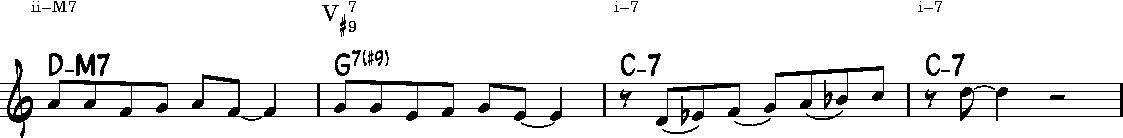
\includegraphics[width=.9\linewidth]{c_min_1.pdf}
\label{orgb0be451}
\end{center}
\subsection{D-7 ii-V-I with minMaj7 -- H/W dim --> min7}
\label{sec:orge3a4c0f}
\begin{center}
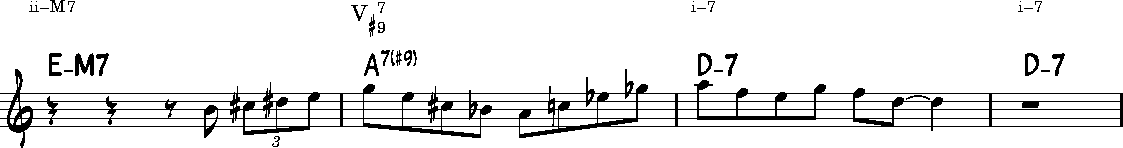
\includegraphics[width=.9\linewidth]{d_min_1.pdf}
\label{org3940de8}
\end{center}
\subsection{D-7 ii-V-I with minMaj7 -- H/W dim --> min7}
\label{sec:org1f2f4c5}
\begin{center}
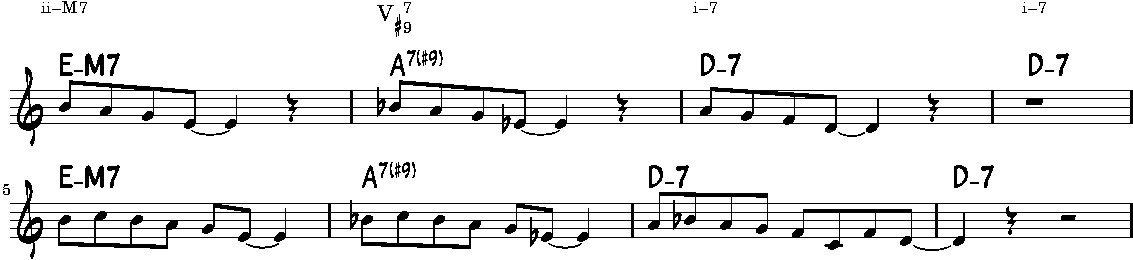
\includegraphics[width=.9\linewidth]{d_min_2.pdf}
\label{orga8813b4}
\end{center}
\subsection{D-7 ii-V-I with minMaj7 -- H/W dim --> min7}
\label{sec:org4eee215}
\begin{center}
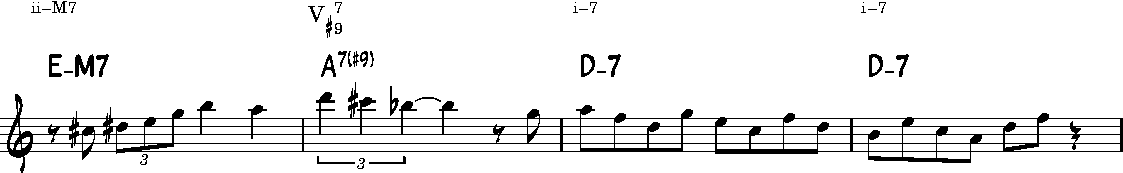
\includegraphics[width=.9\linewidth]{d_min_3.pdf}
\label{org2c3e849}
\end{center}
\subsection{D-7 ii-V-I with minMaj7 -- H/W dim --> min7}
\label{sec:org90abb6f}
\begin{center}
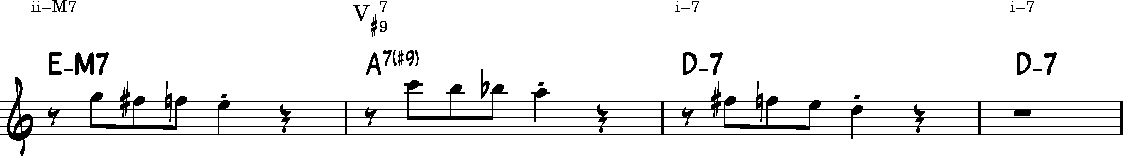
\includegraphics[width=.9\linewidth]{d_min_4.pdf}
\label{orgb5ea3f6}
\end{center}
\subsection{C-7 ii-V-I with minMaj7 -- H/W dim --> min7}
\label{sec:org5fd9dd0}
Type some stuff here

\begin{center}
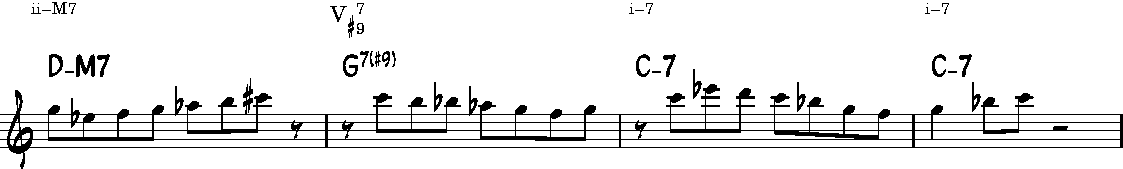
\includegraphics[width=.9\linewidth]{c_min_2.pdf}
\label{orgb39c355}
\end{center}
\subsection{D-7 ii-V-I with minMaj7 -- H/W dim --> min7}
\label{sec:org4d2ff21}
\begin{center}
\includegraphics[width=.9\linewidth]{d_min_5.pdf}
\label{orgefc4911}
\end{center}
\end{document}
